%%%%%%%%%%%%%%%%%%%%%%%%%%%%%%%%%%%%%%%%%
% Beamer Presentation
% LaTeX Template
% Version 1.0 (10/11/12)
%
% This template has been downloaded from:
% http://www.LaTeXTemplates.com
%
% License:
% CC BY-NC-SA 3.0 (http://creativecommons.org/licenses/by-nc-sa/3.0/)
%
%%%%%%%%%%%%%%%%%%%%%%%%%%%%%%%%%%%%%%%%%

%----------------------------------------------------------------------------------------
%	PACKAGES AND THEMES
%----------------------------------------------------------------------------------------

\documentclass{beamer}

\mode<presentation> {

% The Beamer class comes with a number of default slide themes
% which change the colors and layouts of slides. Below this is a list
% of all the themes, uncomment each in turn to see what they look like.

%\usetheme{default}
%\usetheme{AnnArbor}
%\usetheme{Antibes}
%\usetheme{Bergen}
%\usetheme{Berkeley}
%\usetheme{Berlin}
%\usetheme{Boadilla}
%\usetheme{CambridgeUS}
%\usetheme{Copenhagen}
%\usetheme{Darmstadt}
%\usetheme{Dresden}
%\usetheme{Frankfurt}
%\usetheme{Goettingen}
%\usetheme{Hannover}
%\usetheme{Ilmenau}
%\usetheme{JuanLesPins}
%\usetheme{Luebeck}
\usetheme{Madrid}
%\usetheme{Malmoe}
%\usetheme{Marburg}
%\usetheme{Montpellier}
%\usetheme{PaloAlto}
%\usetheme{Pittsburgh}
%\usetheme{Rochester}
%\usetheme{Singapore}
%\usetheme{Szeged}
%\usetheme{Warsaw}

% As well as themes, the Beamer class has a number of color themes
% for any slide theme. Uncomment each of these in turn to see how it
% changes the colors of your current slide theme.

%\usecolortheme{albatross}
%\usecolortheme{beaver}
%\usecolortheme{beetle}
%\usecolortheme{crane}
%\usecolortheme{dolphin}
%\usecolortheme{dove}
%\usecolortheme{fly}
%\usecolortheme{lily}
%\usecolortheme{orchid}
%\usecolortheme{rose}
%\usecolortheme{seagull}
%\usecolortheme{seahorse}
%\usecolortheme{whale}
%\usecolortheme{wolverine}

%\setbeamertemplate{footline} % To remove the footer line in all slides uncomment this line
%\setbeamertemplate{footline}[page number] % To replace the footer line in all slides with a simple slide count uncomment this line

%\setbeamertemplate{navigation symbols}{} % To remove the navigation symbols from the bottom of all slides uncomment this line
}

\usepackage{graphicx} % Allows including images
\usepackage{booktabs} % Allows the use of \toprule, \midrule and \bottomrule in tables

%----------------------------------------------------------------------------------------
%	TITLE PAGE
%----------------------------------------------------------------------------------------

\title[Optimization in Real-Time Signal Processing ]{Convex Optimization in Real Time Signal Processing} % The short title appears at the bottom of every slide, the full title is only on the title page

\author{Adithya Hosapate \\ Sushant Meena} % Your name
\institute[IITH] % Your institution as it will appear on the bottom of every slide, may be shorthand to save space
{
IIT Hyderabad \\ % Your institution for the title page
\medskip
\textit{ee16btech11040@iith.ac.in} % Your email address 
\medskip \\
\textit{es16btech11021@iith.ac.in}
}
\date{\today} % Date, can be changed to a custom date

\begin{document}

\begin{frame}
\titlepage % Print the title page as the first slide
\end{frame}



%----------------------------------------------------------------------------------------
%	PRESENTATION SLIDES
%----------------------------------------------------------------------------------------

%------------------------------------------------


\begin{frame}
\frametitle{Disciplined Convex Programming}
Consider the following optimization problem:\\
\begin{center}
    $\min x^{T}Qx $\\
    subject to $|x_i|\leq 1 $\\
    $\sum x_{i}=10$\\
    $Ax \geq 0$
\end{center}
This problem is not in standard QP form, however it can be easily transformed to standard form by hand.\\

\begin{center}
    $\min x^{T}Qx $\\
    subject to $x_i\leq 1 $\\
    $-x_i\leq -1 $\\
    $\sum x_{i}=10$\\
    $-Ax \leq 0$
\end{center}



\end{frame}




%------------------------------------------------

\begin{frame}

\frametitle{DCP(Continued)}
\begin{itemize}
    \item Recently developed parser-solvers, such as YALMIP, CVX, CVXMOD and Pyomo automate this reduction process.
    \item The user specifies the problem in a natural form by declaring optimization variables, defining an objective, and specifying constraints.
    \item The parser can easily verify convexity of the problem and
automatically transform it to a standard form, for transfer to the solver.
\end{itemize}
\








\end{frame}


%------------------------------------------------



%------------------------------------------------


%----------------------------------------------------------------------------------------

\begin{frame}
\frametitle{Example code}

A = [...]; b = [...]; Q = [...];\\
cvx begin\\
\: variable x(5)\\
\:  minimize (quad form(x, Q))\\
    subjectto\\
        abs(x) \leq 1; sum(x) == 10; A*x \geq 0\\
cvx end\\
cvx status\\

\end{frame}
%----------------------------------------------------------------------------------------

%----------------------------------------------------------------------------------------

\begin{frame}
\frametitle{Kalman Filter}
Kalman filtering is a well-known and widely used method for
estimating the state of a linear dynamical system driven by
noise. When the process and measurement noises are IID Gaussian, the Kalman filter recursively computes the posterior distribution of the state, given the measurements.
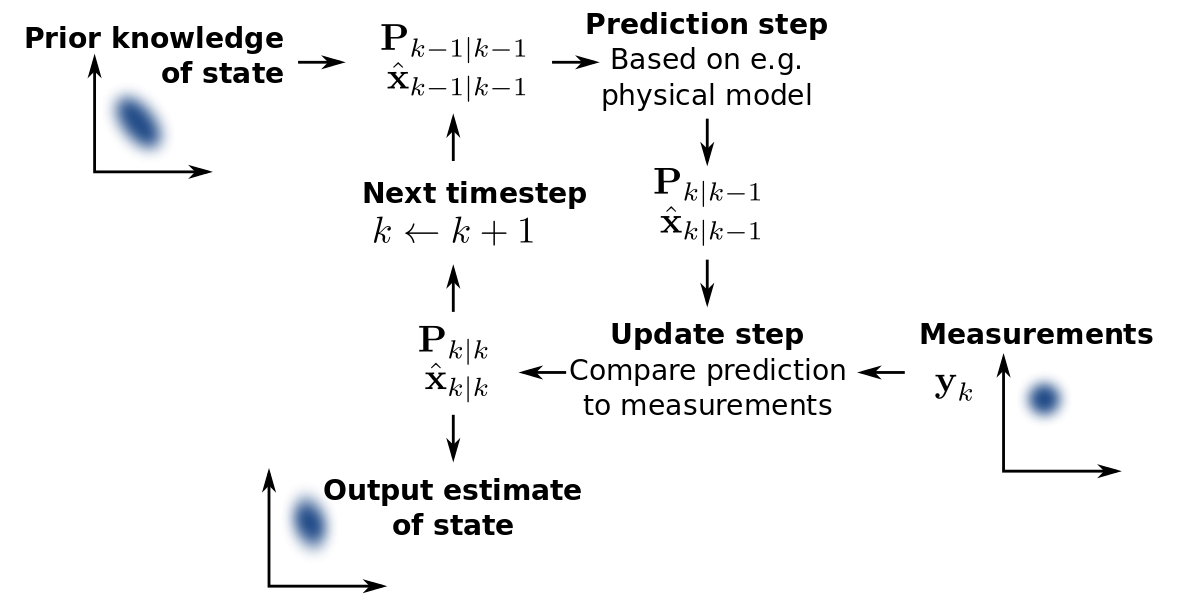
\includegraphics[scale=0.25]{Kalman.png}


\end{frame}
\begin{frame}
\frametitle{Kalman Filter}

We will work with the system:
        $x_t+1 = Ax_t + w_t$ and $y_t = Cx_t + v_t + z_t$,
where $x_{t}$ is the state to be estimated and $y_t$ is the measurement available to us at time step t. Process noise $w_t$ is IID N(0, W) and the measurement noise term $v_t$ is IID N(0, V). The term $z_t$ is an additional noise term, which we assume is sparse and centered around zero.



Alternating time and measurement updates in standard Kalman filter are as follows:

The time update is:\\
\begin{center}
            $\hat{x}_{t|t-1} = A\hat{x}_{t-1|t-1}$
\end{center}
    
and the measurement update is:\\
\begin{center}

    $\hat{x}_{t|t} = \hat{x}_{t|t-1} + \sum C^T(C\sum C^T + V)^{-1}(y_t - C\hat{x}_{t|t-1})$.
\end{center}
\end{frame}

\begin{frame}
\frametitle{Robust Kalman Filter}

We consider a variation on the Kalman filter, designed to handle an additional measurement noise term that is sparse, i.e., whose components are often zero.\\
This term can be used to model (unknown) sensor failures,
measurement outliers, or even intentional jamming. 

Standard Kalman filter requires the solution of a quadratic optimization problem at each step, and has an analytical solution expressible
using basic linear algebra operations.\\

We note that $\hat{x}_{t|t}$ is the solution to the following optimization problem.

\begin{center}
    

\begin{equation*}
    \min v_{t}^T V^{-1}v_{t}+ (x-\hat{x}_{t|t-1})^T \Sigma^{-1}(x-\hat{x}_{t|t-1})+ \lambda ||z_t|| \\
    
   
    s.t \: y_t=Cx+v_t+z_t
\end{equation*}
\end{center} 

\end{frame}

\begin{frame}
\frametitle{Robust Kalman Filter}
This can be rewritten (with appropriate substitution) as
\begin{equation*}
    \min_{z_t} (e_t-z_t)^T Q(e_t-z_t)+ \lambda ||z_t|| 
\end{equation*}
Using the cholesky decomposition of $Q=L^T L$, we can rewrite the optimization problem as\\
\begin{equation*}
    \min_{z_t} ||L(e_t-z_t)||^2 + \lambda ||z_t|| 
\end{equation*}

\begin{equation*}
    \min_{z_t} ||L z_t -L e_t||^2 + \lambda ||z_t|| 
\end{equation*}

On inspection, this is similar to LASSO:\\ 
\begin{equation*}
    \min_{x} ||Ax -b||^2 + \lambda ||x|| 
\end{equation*}

This is very easy to solve using CVXPY as an unconstrained optimization problem.

\end{frame}




\begin{frame}

 In the robust Kalman filter we utilize this optimization for the measurement update, and keep the time update the same as before.

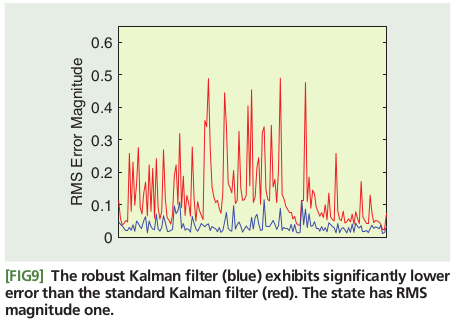
\includegraphics[scale=0.7]{performance.png}

\end{frame}

\end{document} 